\documentclass[12pt]{article}

\usepackage[utf8]{inputenc}
\usepackage{multicol}
\usepackage{geometry}
\usepackage{enumitem}
\usepackage{graphicx}

\author{Ș.l. dr. ing. Robert Lupu (coordonator)\\Petru Dimitriu, Sebastian Scînteie, Tudor-Andrei Vrabie}
\title{Titlu}
\geometry{textheight=700pt}

\begin{document}
	\maketitle
	
	\begin{multicols}{2}
	\subsection*{Introducere}
	Electrooculografia reprezintă o tehnică de măsurare a tensiunii electrice la nivelul corneei dintre partea din față și cea din spate a ochiului uman, semnalul rezultant purtând numele de electrooculogramă.
	
	Prin procesarea adecvată a datelor obținute în cadrul acestui proces se pot determina informații precum direcția privirii, clipitul, gradul de deschidere a ploapelor, etc.
	
	Modalitățile alternative de interacțiune între om și calculator se bucură de un interes crescut atât din partea lumii științifice cât și din partea celei medicale. Pe lângă elementul de noutate pe care îl prezintă, acestea vin în ajutorul persoanelor cu deficiențe sau dizabilități fizice, ușurându-le traiul zilnic dar și facilitând recuperarea persoanelor ce au suferit vătămări ale sistemului neuromotor.
	
	Această lucrare are ca obiectiv expunerea unei modalități de procesare a datelor unei electrooculograme în scopul realizării unei interfețe alternative om-calculator, prin mișcările ochilor. Astfel, s-a încercat modificarea poziției indicatorului mausului pe ecranul unui calculator în concordanță cu deplasarea ochilor.
	
	\subsection*{Detaliile implementării}
	\subsubsection*{Pregătirea măsurătorii}
	Pentru realizarea achiziției de date s–a folosit un dispozitiv (???). Acesta este prevăzut cu (???)
	
	Datele au fost memorate pentru procesare ulterioară folsind mediul MATLAB/Simulink.
	
	Pregătirea dispozitivului pentru utilizare presupune aplicarea electrozilor pe fața persoanei pentru care se realizează măsurători, într-o aranjare bine stabilită. Corespunzător cu cele două canale de date pe care le furnizează, electrozii sunt numerotați 1+, 1-, 2+, 2- și 0, cel din urmă fiind electrodul utilizat drept masă în cadrul măsurătorilor. Așezarea electrozilor s-a realizat astfel:
	\begin{itemize}
		\item [0] pe frunte
		\item [1+] sub ochiul drept
		\item [1-] 
	\end{itemize}
	\subsubsection*{Realizarea măsurătorii}
	Folosind Simulink și modulele aferente dispozitivului, s-au realizat 2 măsurători, achiziționând valorile furnizate de dispozitiv și stocându-le într-un fișier  {\tt.mat}, pentru a putea fi utilizate în cadrul unor simulări ulterioare.
	
	De fiecare dată, s-a avut în vedere eliminarea unei perioade inițiale de 5 secunde pentru a permite atingerea regimului staționar al semnalului furnizat imediat după pornirea achiziției.
	
	Următoarele (???) secunde au ca scop realizarea unei calibrări a dispozitivului. În timpul acesteia, utilizatorul este instruit să privească anumite puncte de pe ecranul monitorului timp de 10 secunde, pentru a se realiza o medie a valorii semnalului obținut, ce va fi utilizată la realizarea unei transformări fereastră-poartă.
	
	Valorile din următoarele secunde reprezintă mișcările propriu-zise ce se vor a fi traduse în deplasări ale indicatorului mausului pe ecran, folosind pentru calibrare valorile obținute anterior.
	
	În scopuri practice și experimentale, s-au reținut mediile semnalelor obținute în urma calibrării și s-au folosit drept constante pentru testarea rezultatelor obținute pentru întregul set de date achiziționat.
	
	\subsection* {Procesarea datelor brute}
	Procesarea datelor brute a avut ca scop:
	\begin{itemize}[noitemsep,nolistsep]
		\item eliminarea zgomotului
		\item eliminarea unui trend general semnalului provenit
		\item simplificarea semnalului pentru obținerea de deplasări uniforme ale indicatorului mausului
	\end{itemize}
	
	Pentru procesarea s-a realizat un filtru după cum astfel. 
	
	\end{multicols}
	
	\begin{multicols}{2}
	Pentru procesare, s-a utilizat o fereastră de 0,5 secunde, adică 128 de eșantioane de date.
	
	De asemenea, s-au utilizat, pentru fiecare canal, o \textit{valoare de prag} și un raport subunitar, numit \textit{fracție}.
	
	Algoritmul de procesare a fost adaptat pentru a permite filtrarea semnalului primit în direct de la dispozitiv, și lucrează cu o fereastră de date ce conține ultimele 128 de eșantioane valorice înregistrare.
	
	Valorile semnalului filtrat se calculează astfel:
	\end{multicols}
	\begin{equation}
	out_{n+1}=\left\{
	\begin{array}{@{} l c @{}}
	out_{n+1} = out_n + 1, y_n > M_i + t \mbox{ și} \left\lfloor y_n - y_{i-128 \cdot f} \right\rfloor > t\\
	out_{n+1} = out_n - 1, y_n < M_i - t \mbox{ și} \left\lfloor y_n - y_{i-128 \cdot f} \right\rfloor > t\\
	out_{n+1} = out_n, \mbox{altfel}
	\end{array}\right.
	\label{eq4}
	\end{equation}
	\begin{multicols}{2}
	În ecuația 1, $out_{n+1}$ reprezintă valoarea curentă a semnalului filtrat, $out_n$ reprezintă valoarea valoarea imediat precedentă a semnalului calculat, $M_i$ reprezintă media aritmetică a valorilor eșantionului curent, $t$ reprezintă valoarea de prag, iar $f$ este fracția amintită mai sus.
	
	Deoarece valorile obținute, cât și comportamentul semnalului diferă între cele două canale, s-au folosit valori diferite ale variabilelor $f$ și $t$ pentru cele două canale, și anume:
	\begin{itemize}[noitemsep, nolistsep]
		\item pentru canalul 1: $t = 45, f = \frac{1}{6}$
		\item pentru canalul 2: $t = 67, f = \frac{1}{8}$
	\end{itemize}
	\end{multicols}
	
	\begin{figure}[h]
		\caption {Semnalele pentru cele două canale, corespunzătoare unui set de date, în forma brută, respectiv procesată}
		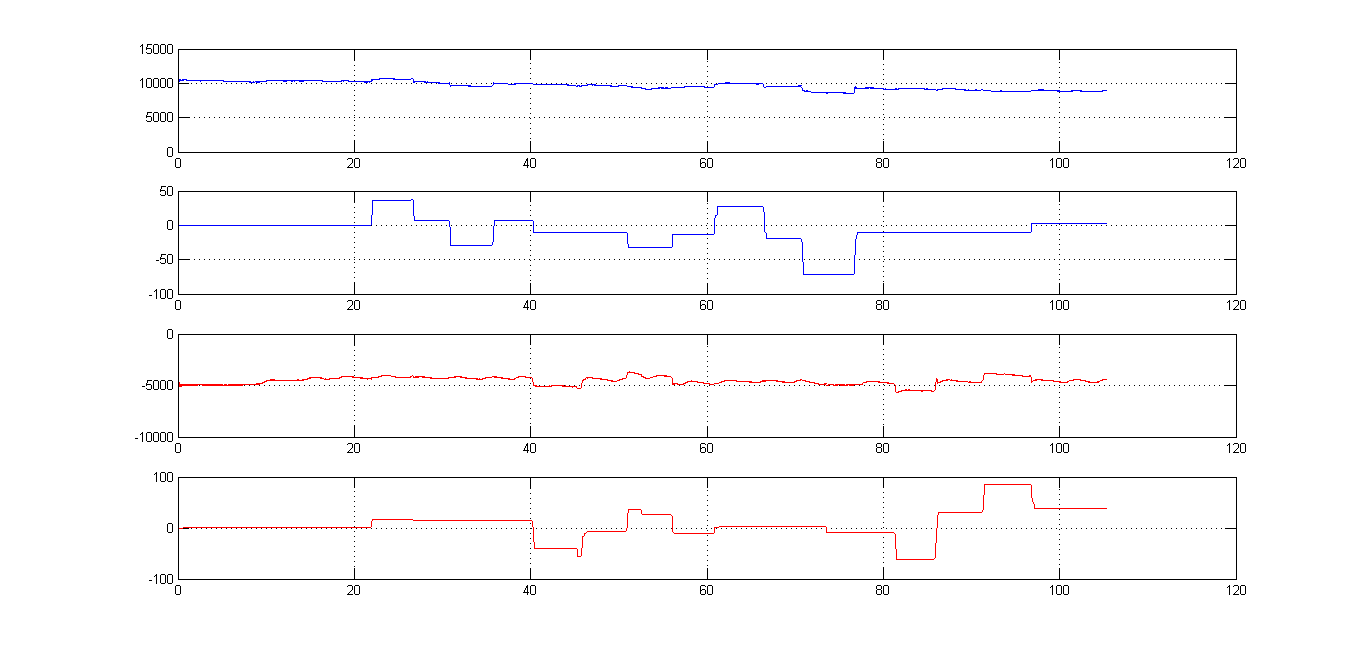
\includegraphics[width=\textwidth]{graph}	
	\end{figure}
	
\end{document}